\section{Полученные результаты}

\label{NeuRadres}

Форма полученных сигналов не была похожа на теоретически ожидаемую (см. Рис.\ref{ris:signal1}). Это можно объяснить множеством физических эффектов, таких, как: фотоны внутри волокна могут испытывать многократное отражение от его границ; в результате отражений фотоны могут попасть на пиксель, несоответствующий волокну, в котором они родились; несмотря на все нанесённые светоизолирующие покрытия на поверхности каждого волокна, остаётся вероятность прохождения фотонов из одного волокна в другое.

Несмотря на достаточно необычную форму сигналов, вероятнее всего сигналы состоят из совокупности так называемых одноэлектронных сигналов. Одноэлектронным сигналом будем называть сигнал, возникающий на аноде ФЭУ в результате выбивания одного электрона с фотокатода. Поэтому суммарный вид сигналов принял привычную форму, из которой было определено, что время высвечивания равно 5,8\,нс, для данного сцинтиллятора которое равняется 3,2\,нс \cite{crystals}.

\begin{figure}[h]
	\center{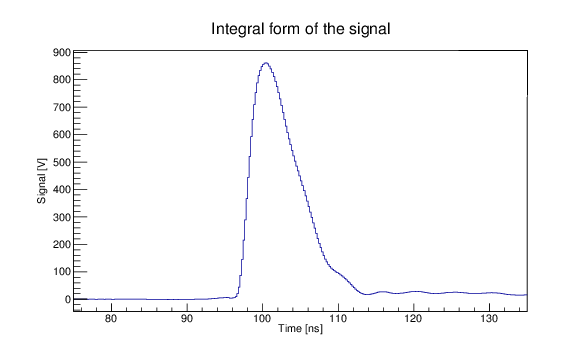
\includegraphics[width=1\linewidth]{integralform.png}}
	\caption{Суммарный сигнал с одного канала.}
	\label{ris:integralform}
\end{figure}

Очевидно, величина $\Delta\tau$ (см. уравнение \eqref{koordinate}) зависит от множества случайных процессов, таких, как: продольная координата взаимодействия падающей частицы с материалом детектора, энергия электрона отдачи, количество испущенных сцинтиллятором фотонов, достигнувших фотокатода ФЭУ и других. Форма распределения этой величина ожидалась схожей формой нормального распределения случайной величины. Поэтому временное разрешение прототипа детектора NeuRad оценивалось как параметр полной ширины на половине высоты (англ. FWHM - full width at half maximum) распределения разницы времён сигналов ($\Delta\tau$) с противоположных сторон одного оптического волокна.

Параметр FWHM вычислялся по формуле:
\begin{equation}
\label{FWHM}
{\rm FWHM}=2\sqrt{2\ln(2)}\sigma,
\end{equation}
где $\sigma$ - есть стандартное отклонение, которое рассчитывалось фитированием формы распределения $\tau$ функцией Гаусса~\cite{vratislav}. 
Параметры методов расчёта времени сигналов подбирались таким образом, чтобы FWHM распределения $\Delta\tau$ было наименьшим. 

\begin{figure}[!ht]
	\centering
	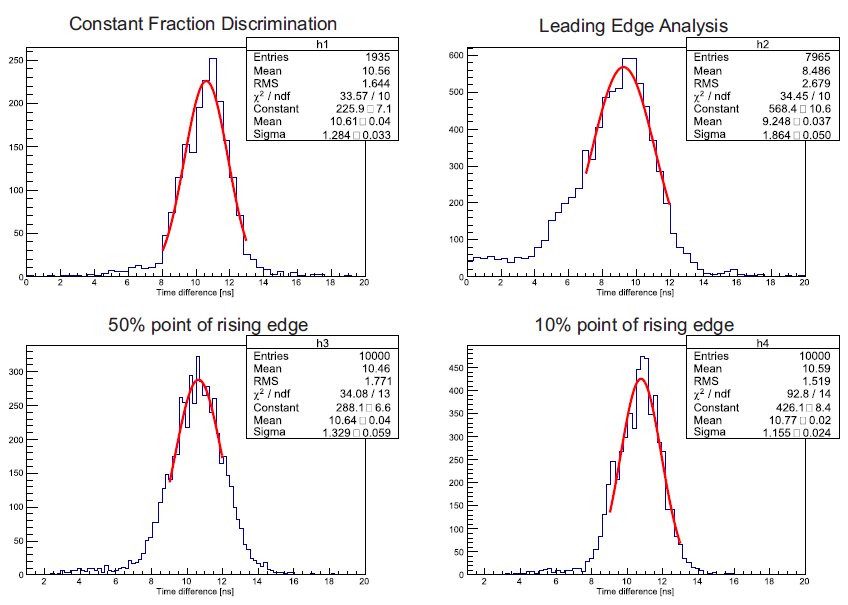
\includegraphics[width=1\linewidth]{tau.png}
	\captionof{figure}{Распределение $\Delta\tau$ для сигналов с противоположных сторон одного оптического волокна.}
	\label{ris:Tau}
\end{figure}

На Рис.\ref{ris:Tau} показаны распределения $\Delta\tau$, рассчитанное с помощью методов описанных в главе\,\ref{section:processing}. Хотя пучок был коллимирован посередине продольной длины детектора, математическое ожидание (Mean) всех распределений принимает значение около 10\,нс. Это объясняется тем, что кабеля для снятия сигналов с ФЭУ были разной длины, и разница времени задержки сигналов была равна 10\,нс. 

Слева вверху (Constant Fraction Discriminator): распределение $\Delta\tau$, разницы времён сигналов с противоположных сторон одного оптического волокна, рассчитанное методом CFD с параметрами: время задержки 1.5 нс, коэффициент ослабления инвертированного сигнала  0.3.
Справа вверху (Leading Edge Analysis): $\Delta\tau$ рассчитано методом LED с порогом 10\,mV. 
Внизу : $\Delta\tau$ рассчитано методом анализа переднего фронта сигнала с порогом 10 mV. Время сигнала рассчитывали, как момент достижения 50\%(слева) и 10\%(справа) амплитуды первого локального максимума.
 
\begin{table}[!t]
	\centering
	\begin{tabular}{|c|c|c|c|}
		\hline
		\textbf{Метод}: & \textbf{Параметры} & $\sigma$\,[нс] & FWHM\,[нс]\\
		\hline
		CFD & Задержка  1,5\,нс & 1,28 & 3,02 \\
		 & коэффициент ослабления 0,3 &  & \\
		\hline
		LED & Порог 20\,мВ &  1,86 & 4,39\\
		\hline
		Анализ фронта 50\% & Порог 20\,мВ &  1,33 & 3,13\\
		\hline
		Анализ фронта 10\% & Порог 20\,мВ &  1,16 & 2,72\\
		\hline
	\end{tabular}
	\caption{ Результаты рассчётов временного разрешения прототипа NeuRad.}\label{tab:results}
\end{table}

Временное разрешение, полученное из распределений на Рис.\ref{ris:Tau} показано в таблице~\ref{tab:results}. Поскольку полученные значения не удовлетворили ожиданиям, мы приступили к анализу отбора событий и корректировки сигналов. 

Была замечена сильная зависимость $\Delta\tau$ для метода CFD от суммарного заряда, регистрируемых ФЭУ с двух сторон оптического волокна, см. Рис.\ref{ris:walk}а). Очевидно, что такая зависимость является следствием не физических явлений, а свойством записи данных.

\begin{figure}[!ht]
	\centering
	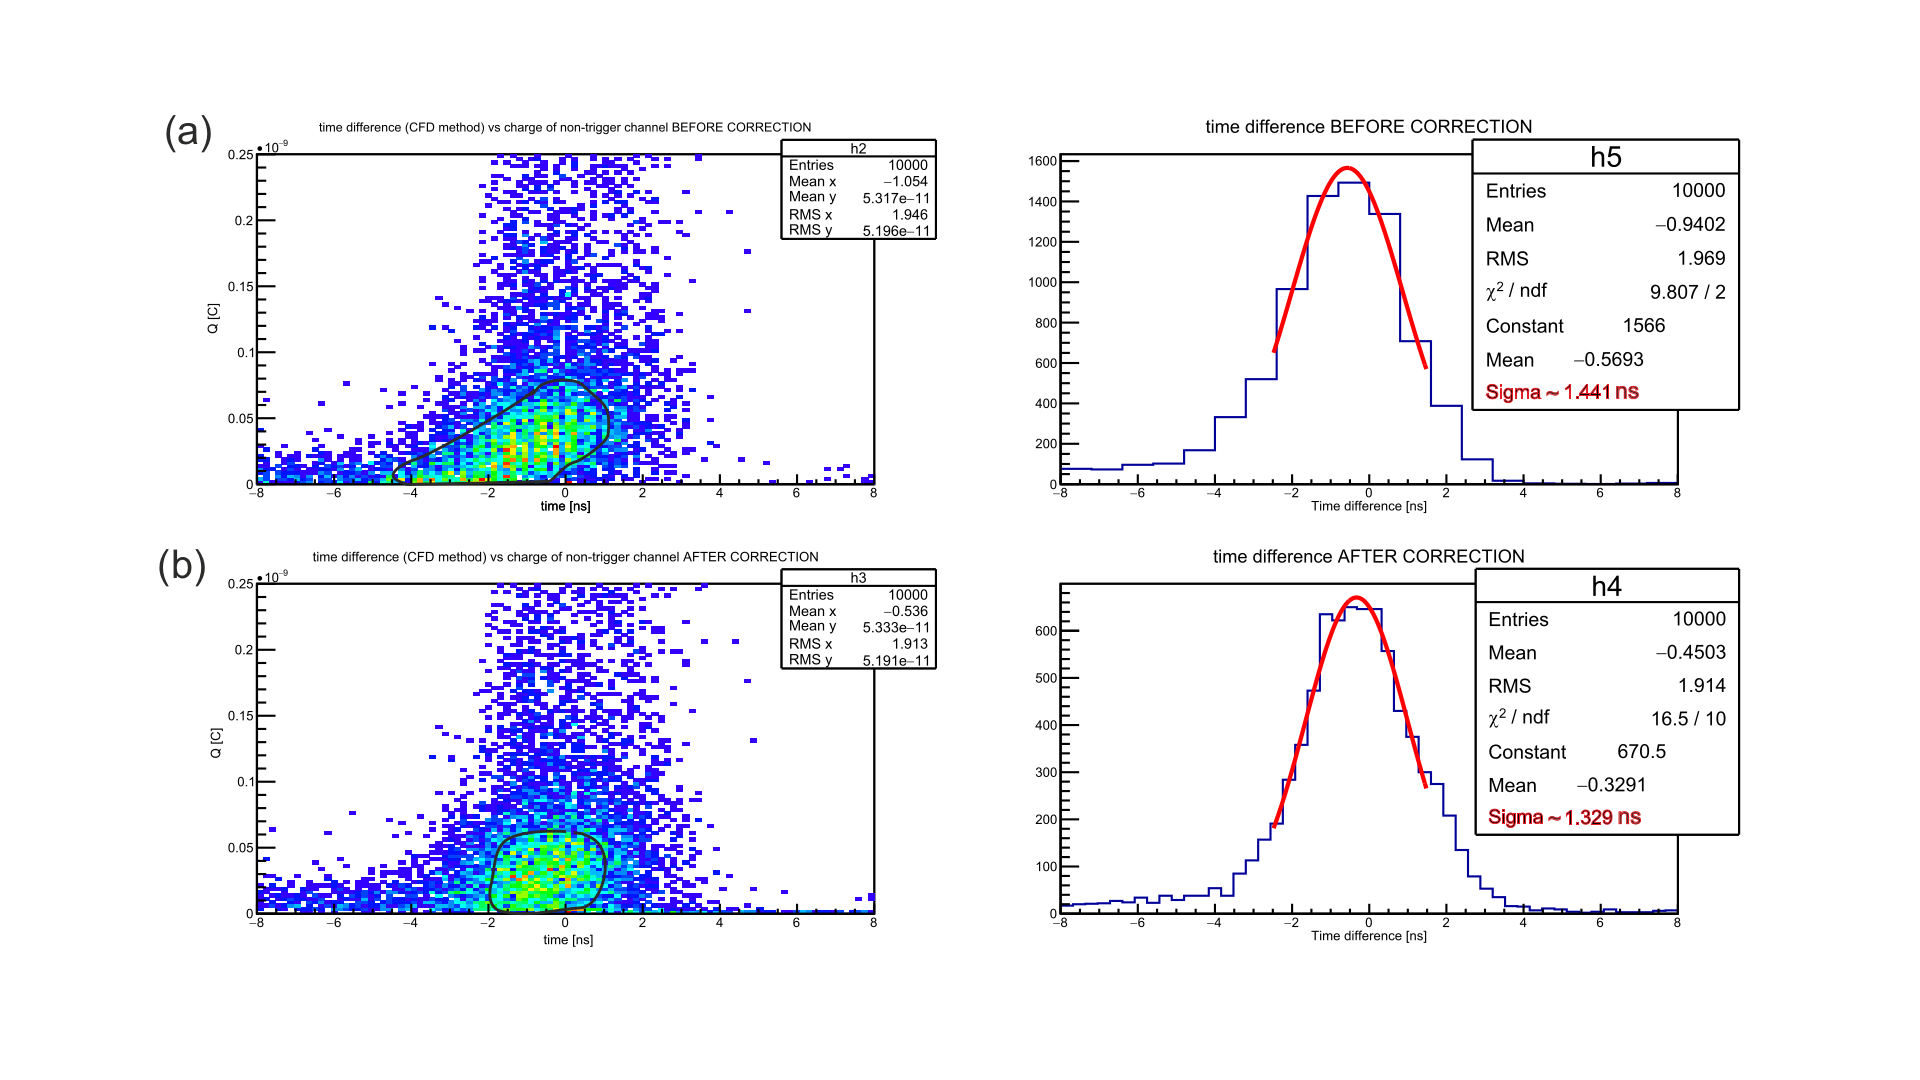
\includegraphics[width=1.0\linewidth]{walkcorr.png}
	\caption{В левом столбце показана зависимость $\Delta\tau$ (с помощью метода CFD) от заряда, в правом столбце проекция на ось $\Delta\tau$. а) Экспериментальные данные без коррекции. b) Экспериментальные данные после корректировки.}
	\label{ris:walk}
\end{figure}

Поэтому, полученный параметр $\Delta\tau$ был скорректирован так, чтобы максимально уменьшить визуально очевидную зависимость $\Delta\tau$ от заряда. Для этого, каждое рассчитанное $\Delta\tau$ изменялось следующим образом:
\begin{equation}
\Delta\tau' = \Delta\tau + \frac{k}{Q},
\end{equation}
где $\Delta\tau'$ - новое, скорректированное значение разницы времён, $Q$ - заряд, $k$ - коэффициент корректировки, подбирающийся так, чтобы в результате корректировки минимизировать зависимость разницы времён сигналов от заряда. В корректировке, показанной на Рис.\ref{ris:walk}, $k$ был равен 2\,нс.
На Рис.\ref{ris:walk}b) показана зависимость $\Delta\tau'$ от заряда, получившаяся в результате корректировки и распределение $\Delta\tau'$. 

Вторым методом уменьшения значения временного разрешения был отбор событий. Как описывалось выше, наиболее интересными являются сигналы с большой максимальной амплитудой и, соответственно, большим регистрируемым зарядом и длинными по времени. Наиболее удачным параметром для отбора был выбран параметр Time-over-Threshold(ToT), который рассчитывался, как разница времён пересечения сигнала уровня, равного половине максимальной амплитуды сигнала, заднего и переднего фронтов сигнала.

\begin{figure}[!h]
	\centering
	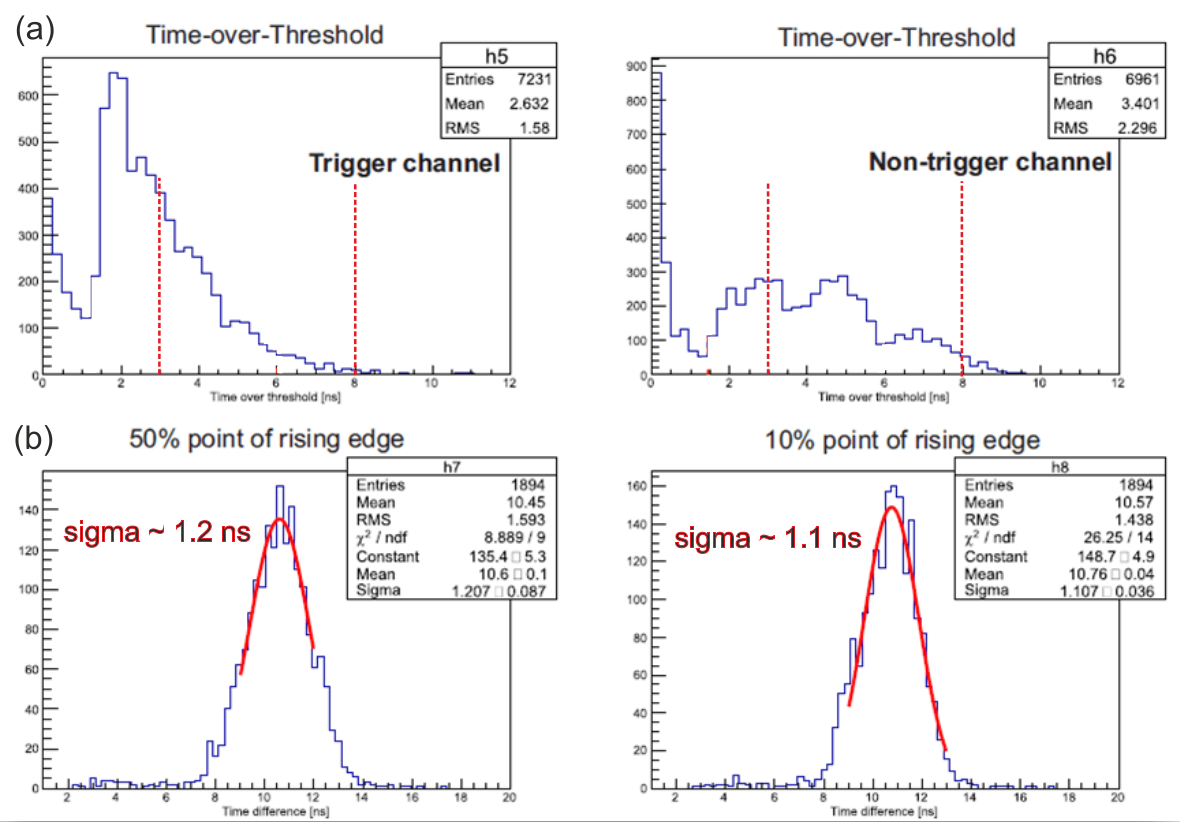
\includegraphics[width=0.8\linewidth]{totcorr.png}
	\caption{а) Распределение ToT для двух каналов одного оптического волокна. b) Распределение разницы времён сигналов для событий, удовлетворяющих условию отбора. }\label{ris:totcorr}
\end{figure}

На Рис.\ref{ris:totcorr} показано распределение параметра ToT для двух рассматриваемых каналов, $\Delta\tau$ после отбора. Условие отбора заключается в том, что для рассматриваемых событий ToT должен быть больше 3, но меньше 8\,нс.
Таким образом, лучшая оценка временного разрешения детектора была рассчитана методом анализа переднего фронта сигнала с привязкой к точке 10\% амплитуды от максимальной \red{и равно 2,59\,нс}. Такой временная неопределённости детектирования падающей частицы соответствует неопределённости по координате 47\,см, см. формулу\,\ref{eq:distance}. 

\subsection{Эксперимент с пластиной сцинтиллятора в GSI}

Все методы описанные в выше были применены для данных, собранных на установке на территории GSI.

Полученные результаты описывающие временные характеристики изображены на Рис.~\ref{ris:GSIcfd_amp}. Как и ожидалось, временное разрешение такой установки лучше, чем разрешение прототипа NeuRad, так как в данном случае отсутствует вклад пространственного разрешения из-за малого размера чувствительной части детектора.

В верхней части рисунка~\ref{ris:GSIcfd_amp} изображены распределения разницы времён сигналов, рассчитанное методом диксриминатора со следящим порогом до отбора по параметру ToT слева и после отбора справа. Данный отбор являлся наиболее удачным для набранных данных, о чём свидетельствует нижняя часть рисунка. В нижней части изображена зависимость суммы максимальных амплитуд сигналов в двух каналов от $\Delta\tau$. Визуально очевидно, что данный отбор отсеивает подавляющее большинство событий, c отклонённым значением $\Delta\tau$ от ожидаемой.

\begin{figure}
	\centering
	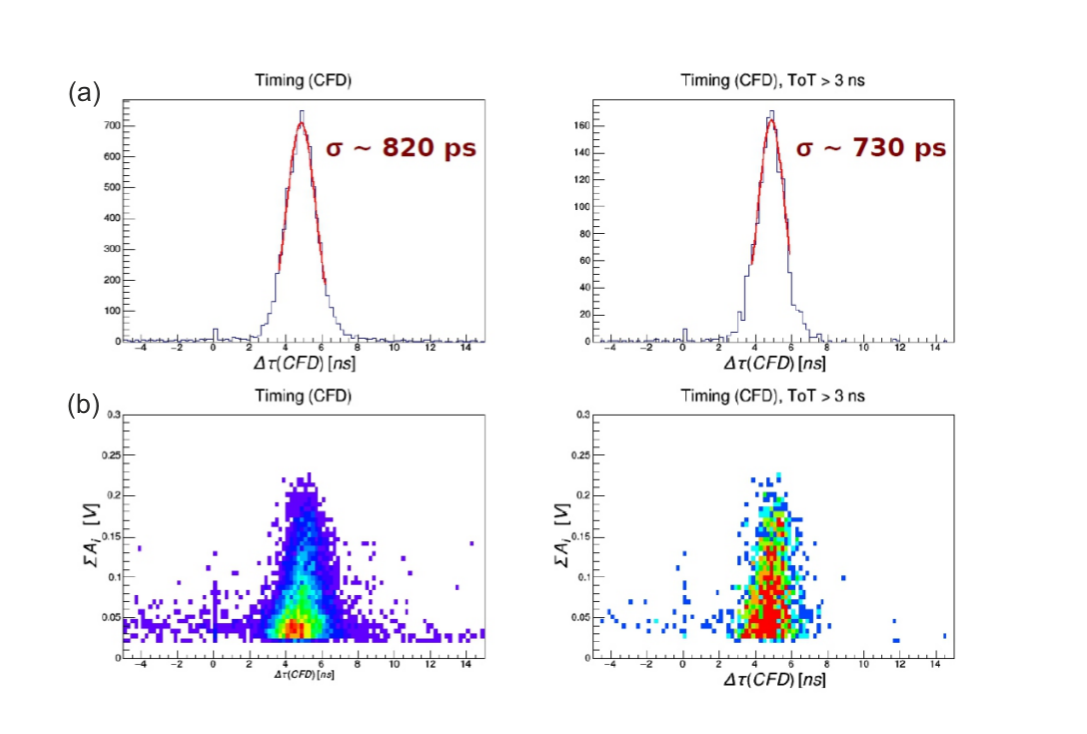
\includegraphics[width=1\linewidth]{CFD_amp.png}
	\caption{Корреляция разницы времён сигналов, оцененных методом CFD, с суммой амплитуд сигналов с эксперимента с пластиной сцинтиллятора. Справа - эта же корреляция, но с отбором событий, для которых время сигнала над порогом больше 3\,нс.}
	\label{ris:GSIcfd_amp}
\end{figure}